\documentclass[aspectratio=169,11pt]{beamer}
\usepackage[utf8]{inputenc}
\usepackage[T1]{fontenc}
\usepackage{lmodern,graphicx,amsmath,amssymb,booktabs,array}
\usepackage{xcolor,tikz}
\usetikzlibrary{arrows.meta,positioning,calc,fit,shapes.geometric,decorations.pathreplacing}

% Visual language follows the supplied research_ideas_hybrid_modeling template.
\definecolor{tumblue}{RGB}{0,101,189}
\definecolor{tumdark}{RGB}{0,51,89}
\definecolor{tumgray}{RGB}{105,105,105}
\definecolor{tumlight}{RGB}{235,243,248}
\definecolor{tumgreen}{RGB}{162,173,0}
\definecolor{tumorange}{RGB}{243,125,32}
\definecolor{tumred}{RGB}{229,52,24}
\definecolor{coffee}{HTML}{6F4E37}
\definecolor{waterblue}{HTML}{66B5D8}
\definecolor{modelgreen}{HTML}{4C956C}
\definecolor{datagray}{HTML}{E8E8E8}

\usetheme{default}
\setbeamertemplate{navigation symbols}{}
\setbeamercolor{normal text}{fg=black,bg=white}
\setbeamercolor{frametitle}{fg=tumblue}
\setbeamercolor{structure}{fg=tumblue}
\setbeamercolor{itemize item}{fg=tumblue}
\setbeamertemplate{itemize items}[circle]
%
\setbeamertemplate{headline}{\leavevmode\begin{beamercolorbox}[wd=\paperwidth,ht=3.2ex,dp=1.6ex]{frametitle}\hfill\raisebox{-0.85cm}{\IfFileExists{figures/tum_logo.png}{
\includegraphics[height=0.8cm]{figures/tum_logo.png}}{\fbox{\scriptsize Add tum\_logo.png}}}\hspace*{1em}\end{beamercolorbox}}
\setbeamertemplate{footline}{%
  \leavevmode\begin{beamercolorbox}[wd=\paperwidth,ht=3.2ex,dp=1.3ex]{author in head/foot}
  \hspace*{1em}\color{tumgray} Khalifa and Briesen \enspace|\enspace FineFlow--Espresso
  \hfill\insertsectionhead\hfill\insertframenumber/\inserttotalframenumber\hspace*{1em}
  \end{beamercolorbox}}

\graphicspath{{figures/}}
\newcommand{\hi}[1]{\textcolor{tumblue}{\textbf{#1}}}
\newcommand{\pos}[1]{\left[#1\right]_+}
\newcommand{\question}[1]{%
  \begin{beamercolorbox}[rounded=true,sep=0.7em]{block body}
    \centering\large\color{tumdark}\textbf{#1}
  \end{beamercolorbox}}
\newcommand{\takeaway}[1]{%
  \begin{beamercolorbox}[rounded=true,sep=.55em]{block body}
    \centering\color{tumdark}\textbf{#1}
  \end{beamercolorbox}}
\newcommand{\slidesource}[1]{\par\vfill{\tiny\color{tumgray}#1}}
\newcommand{\safeimage}[3]{%
  \includegraphics[width=#2,height=#3,keepaspectratio]{#1}}
\tikzset{
  box/.style={draw=tumdark!75,rounded corners=2pt,fill=tumlight,align=center,
    minimum height=9mm,text width=2.55cm,font=\small,inner sep=3pt},
  databox/.style={box,fill=datagray},
  physicsbox/.style={box,fill=waterblue!18},
  outputbox/.style={box,fill=modelgreen!15},
  arr/.style={-{Latex[length=2mm]},thick,tumblue},
  fine/.style={circle,fill=tumorange,draw=tumorange!70!black,inner sep=1.05pt},
  grain/.style={circle,fill=coffee!25,draw=coffee,thick,minimum size=4.8mm}}

% Flexible row/column system retained from the supplied template.
\newcommand{\FlexRowHeight}{}
\newenvironment{FlexRow}[1]{%
 \def\FlexRowHeight{#1}%
 \begin{overlayarea}{\textwidth}{#1}%
  \begin{columns}[T,onlytextwidth]%
}{%
  \end{columns}%
 \end{overlayarea}%
}
\newcommand{\Col}[2]{%
 \column{#1\textwidth}%
 \begin{minipage}[t][\FlexRowHeight]{\linewidth}%
  #2%
 \end{minipage}%
}



\begin{document}

\begin{frame}{}
 \vspace*{0.05cm}
 \begin{center}
  {\Large\bfseries FineFlow--Espresso:}\\[.7ex]
  {\Large\bfseries A Calibratable 1D Model of Fines Migration}
 \end{center}
 \vspace{0.15cm}
 \begin{columns}[c,onlytextwidth]
  \column{0.55\textwidth}
   
   {\color{tumblue}\textbf{A continuum model linking fines transport and hydraulic resistance}}
   
   \vspace{0.7cm}

   Technical University of Munich\\
   Chair of Process Systems Engineering\\[0.55cm]
    Ali Khalifa \& Heiko Briesen 
  \column{0.41\textwidth}\centering
   \safeimage{figures/uhrenturm.jpg}{1.05\linewidth}{4.5cm}
 \end{columns}
\end{frame}

\begin{frame}{Presentation outline}
\tableofcontents
\end{frame}

\section[Motivation]{Motivation and research question}
\begin{frame}{}
\vfill
{\large\color{tumgray}Section 1 of 7}\par\vspace{0.4cm}
{\LARGE\color{tumblue}\textbf{Motivation and research question}}\par\vspace{0.5cm}
{\large How do fines change resistance and cup washout?}
\vfill
\end{frame}

\begin{frame}{Motivation and research question}
\hi{Can a 1D model reproduce the experimental response?}
\begin{itemize}
\item Predict the outlet flow rate for the measured pressure drop.
\item Predict the amount of fines reaching the cup.
\end{itemize}
\medskip
\question{How does fines redistribution change the hydraulic resistance and cup washout?}
\medskip
\small Darcy relates pressure to flow through permeability. Deposits change pore space and resistance. Release, capture and remobilization determine the fines distribution.
\end{frame}

\section[Model scope]{Physical mechanisms and model scope}
\begin{frame}{}
\vfill
{\large\color{tumgray}Section 2 of 7}\par\vspace{0.4cm}
{\LARGE\color{tumblue}\textbf{Physical mechanisms and model scope}}\par\vspace{0.5cm}
{\large Release, capture and remobilization inside the puck}
\vfill
\end{frame}

\begin{frame}{Flow and fines inside the coffee bed}
 \begin{columns}[c,onlytextwidth]
  \column{0.42\textwidth}\centering
   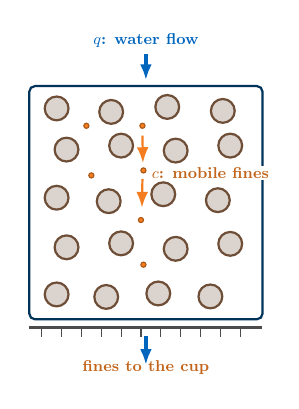
\begin{tikzpicture}[scale=.63,transform shape]
    \draw[rounded corners=2pt,thick,tumdark] (0,0) rectangle (4.7,4.7);
    \draw[arr,line width=1.2pt] (2.35,5.35)--(2.35,4.82);
    \node[tumblue,font=\small\bfseries] at (2.35,5.62) {$q$: water flow};
    \foreach \x/\y in {.55/.5,1.55/.45,2.6/.52,3.65/.46,
      .75/1.45,1.85/1.53,2.95/1.42,4.05/1.52,
      .55/2.45,1.6/2.38,2.7/2.52,3.8/2.4,
      .75/3.42,1.85/3.5,2.95/3.4,4.05/3.5,
      .55/4.25,1.65/4.18,2.78/4.28,3.9/4.2}{\node[grain] at (\x,\y) {};}
    \foreach \x/\y in {1.15/3.9,2.28/3.9,2.3/3.0,1.25/2.9,2.25/2.0,2.3/1.1}
      \node[fine] at (\x,\y) {};
    \draw[arr,tumorange] (2.28,3.7)--(2.29,3.15);
    \draw[arr,tumorange] (2.28,2.83)--(2.27,2.25);
    \node[font=\small\bfseries,tumorange!80!black,fill=white,inner sep=1pt]
      at (3.65,2.95) {$c$: mobile fines};
    \draw[very thick,black!70] (0,-.16)--(4.7,-.16);
    \foreach \x in {.25,.65,...,4.45}{\draw[black!70] (\x,-.16)--(\x,-.36);}
    \draw[arr,line width=1.2pt] (2.35,-.34)--(2.35,-.92);
    \node[font=\small\bfseries,tumorange!80!black] at (2.35,-.98) {fines to the cup};
   \end{tikzpicture}
  \column{0.54\textwidth}
   \small
   \hi{Flow and mobile fines}
   \begin{itemize}
    \item $Q$: flow rate; $A$: puck area; $q=Q/A$: superficial velocity;
    \item $c$: mobile-fines concentration; $q\,c$: advective fines flux.
   \end{itemize}
   \hi{Pore structure and retained fines}
   \begin{itemize}
    \item $\varepsilon$: porosity; $K$: permeability;
    \item $m_a$: remaining initially attached fines;\\ $m_d$: recaptured deposits;
    \item $m_a,m_d$: mass per bulk volume; $c$: mass per water volume.
   \end{itemize}
 \end{columns}
\vspace{.12cm}\takeaway{Distinct retained populations assume different kinetics or hydraulic effects.}
 %\vspace{.2cm}
 %\takeaway{$q\,c$ means $q$ multiplied by $c$; $c$ is not a subscript.}
\end{frame}

\begin{frame}{Scope of the 1D continuum model}
\small

\hi{Present approach}
\begin{itemize}
\item Forward flow with cross-section-averaged fields varying in $z$ and $t$.
\item CT stage snapshots can constrain axial structural changes.
\item Pressure and flow histories constrain the evolving total resistance.
\end{itemize}
\medskip
\hi{Limits and next measurements}
\begin{itemize}
\item \textbf{Reverse flow and radial channeling are outside the scope of this work.}
\item CT shows radial heterogeneity. Measurements must test whether axial averaging captures the overall hydraulic response.
\item Time-resolved cup-fines data are a proposed measurement; availability is unconfirmed.
\item Pore networks and 2D/3D continuum models are future extensions.
\end{itemize}

\end{frame}

\begin{frame}{Fines exchange locally and leave through the outlet}
 \centering
 
 \vspace*{0.1cm}
 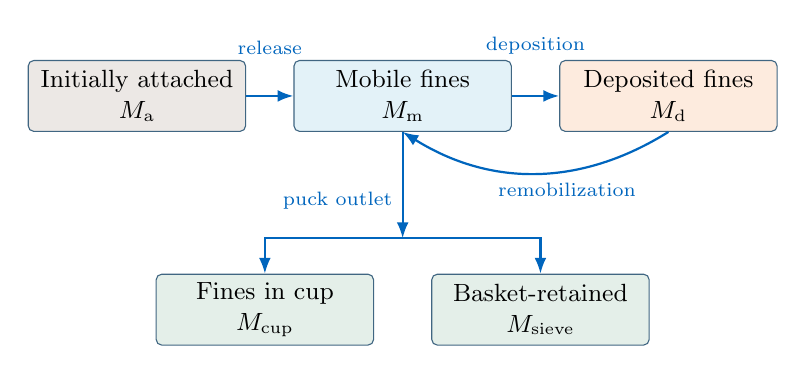
\begin{tikzpicture}[node distance=7mm and 6mm]
  \node[box,fill=coffee!13] (a) {Initially attached\\$M_{\mathrm a}$};
  \node[physicsbox,right=of a] (m) {Mobile fines\\$M_{\mathrm m}$};
  \node[box,right=of m,fill=tumorange!15] (d) {Deposited fines\\$M_{\mathrm d}$};
  \node[outputbox,below=18mm of m,xshift=1.75cm] (s) {Basket-retained\\$M_{\mathrm{sieve}}$};
  \node[outputbox,below=18mm of m,xshift=-1.75cm] (cup) {Fines in cup\\$M_{\mathrm{cup}}$};
  \draw[arr] (a)--node[above=4mm,font=\scriptsize]{release}(m);
  \draw[arr] (m)--node[above=4mm,font=\scriptsize]{deposition}(d);
  \draw[arr] (d.south) to[bend left=32] node[below,,xshift=4mm,font=\scriptsize]{remobilization} (m.south);
  \coordinate (split) at ($(m.south)+(0,-1.35)$);
  \draw[arr] (m.south)--node[left,yshift=-2mm,font=\scriptsize]{puck outlet}(split);
  \draw[arr] (split)-|(cup.north);
  \draw[arr] (split)-|(s.north);
 \end{tikzpicture}
 \vspace{.2cm}
 \[
 M_0=M_{\mathrm a}+M_{\mathrm m}+M_{\mathrm d}+M_{\mathrm{sieve}}+M_{\mathrm{cup}}.
 \]
\centering\small $M_a=A\int m_a\,dz$, $M_m=A\int\varepsilon c\,dz$, $M_d=A\int m_d\,dz$.
 \takeaway{Accounting domain: puck + basket + collected cup fines.}
\end{frame}

\section[Equations]{Governing equations and closures}
\begin{frame}{}
\vfill
{\large\color{tumgray}Section 3 of 7}\par\vspace{0.4cm}
{\LARGE\color{tumblue}\textbf{Governing equations and closures}}\par\vspace{0.5cm}
{\large Balances and constitutive choices for fines and flow}
\vfill
\end{frame}

\begin{frame}{Model overview: pressure, flow and fines reaching the cup}
\centering
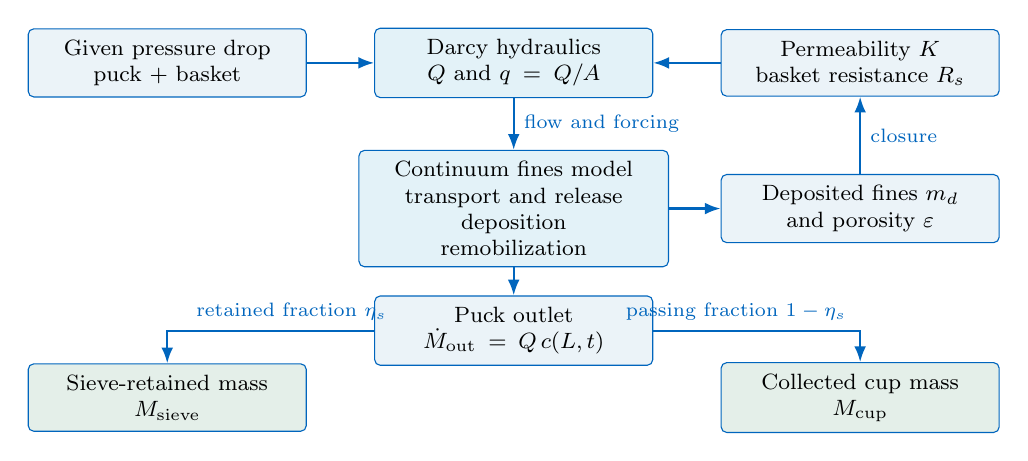
\begin{tikzpicture}[
 overview/.style={draw=tumblue,rounded corners=2pt,fill=tumlight,
 align=center,text width=3.25cm,minimum height=.75cm,font=\footnotesize,inner sep=4pt},
 link/.style={-{Latex[length=2mm]},thick,tumblue}]
\node[overview] (pressure) at (0,0) {Given pressure drop\\puck + basket};
\node[overview,fill=waterblue!18] (darcy) at (4.4,0) {Darcy hydraulics\\$Q$ and $q=Q/A$};
\node[overview] (perm) at (8.8,0) {Permeability $K$\\basket resistance $R_s$};
\node[overview,fill=waterblue!18,text width=3.65cm] (fines) at (4.4,-1.85)
 {Continuum fines model\\transport and release\\deposition\\remobilization};
\node[overview] (deposit) at (8.8,-1.85) {Deposited fines $m_d$\\and porosity $\varepsilon$};
\node[overview] (out) at (4.4,-3.4) {Puck outlet\\$\dot M_{\mathrm{out}}=Q\,c(L,t)$};
\node[overview,fill=modelgreen!15] (sieve) at (0,-4.25) {Sieve-retained mass\\$M_{\mathrm{sieve}}$};
\node[overview,fill=modelgreen!15] (cup) at (8.8,-4.25) {Collected cup mass\\$M_{\mathrm{cup}}$};
\draw[link] (pressure)--(darcy);
\draw[link] (perm)--(darcy);
\draw[link] (darcy)--node[right,font=\scriptsize]{flow and forcing}(fines);
\draw[link] (fines)--(deposit);
\draw[link] (deposit)--node[right,align=left,font=\scriptsize]{closure}(perm);
\draw[link] (fines)--(out);
\draw[link] (out.west)-|node[pos=.2,above,font=\scriptsize]{retained fraction $\eta_s$}(sieve.north);
\draw[link] (out.east)-|node[pos=.2,above,font=\scriptsize]{passing fraction $1-\eta_s$}(cup.north);
\end{tikzpicture}
\par\smallskip\small
Kozeny--Carman uses $\varepsilon(m_d)$ to obtain $K$.
The exponential alternative uses $m_d$ directly.
\end{frame}

\begin{frame}{Darcy flow and the permeability closure have different roles}
\small
\hi{Darcy links the measured pressure drop to outlet flow}
\[
-\frac{\partial p}{\partial z}=\frac{\mu q}{K(z,t)},\qquad q=Q/A.
\]
Lower permeability $K$ means greater resistance and less flow at the same pressure drop.
\[
R_{\mathrm{tot}}=\frac{\mu}{A}\int_0^L\frac{\mathrm dz}{K(z,t)}+R_s,
\qquad Q=\frac{\Delta p_{\mathrm{total}}}{R_{\mathrm{tot}}}.
\]
$R_s$: basket hydraulic resistance [Pa\,s\,m$^{-3}$]. $\mu$: water viscosity.
$\Delta p_{\mathrm{total}}$: pressure drop across puck plus basket.
\par\medskip
\hi{Next: how do deposits change $K$?}
\par The permeability closure describes that structural response. Fines balances then determine how the deposits evolve.
\end{frame}

\begin{frame}{Two alternative closures for the same permeability}
\small
Both closures supply $K$ to Darcy. Deposits reduce the available pore space.
\[\varepsilon=\max\left(\varepsilon_0-m_d/\rho_d,\varepsilon_{\min}\right)\]
$\rho_d$: deposit density. Capture raises $m_d$ and remobilization lowers it.
Initial release affects porosity indirectly through later capture in this model.
\par\smallskip
\begin{columns}[T,onlytextwidth]
\column{.49\textwidth}\hi{Kozeny--Carman: structural baseline}
\[\frac{K}{K_0}=\left(\frac{\varepsilon}{\varepsilon_0}\right)^3
\left(\frac{1-\varepsilon_0}{1-\varepsilon}\right)^2\]
Relates permeability to porosity under fixed effective particle scale and Kozeny factor.
\par\medskip This simplified relation may miss changes in pore connectivity and localized plugging.
\column{.47\textwidth}\hi{Exponential: empirical comparison}
\[\frac{K}{K_0}=\exp\left(-\beta\frac{m_d}{m_{\mathrm{cap}}}\right)\]
Assumes a direct sensitivity to deposit loading. $\beta$ controls the imposed blockage strength.
\par\medskip This empirical law has no coffee-data calibration here.
\end{columns}
\vfill\takeaway{Identical initial $K_0$. Neither closure has experimental validation.}
\end{frame}

\begin{frame}{Why the illustrative model used an exponential law}
\small
\hi{Motivation: represent strong blockage with a simple adjustable law}
\par\medskip
The hypothesis was that fines obstruct narrow flow paths, allowing a large resistance increase with a modest change in total porosity.
\par\medskip
The exponential form stays positive and decreases smoothly. These useful mathematical properties do not establish physical validity.
\medskip
\begin{columns}[c,onlytextwidth]
\column{.45\textwidth}
\begin{tabular}{cc}\toprule
$m_d/m_{\mathrm{cap}}$ & $K/K_0$ at $\beta=5.5$\\\midrule
0 & 1\\[.35em]
0.5 & 0.064\\[.35em]
1 & 0.0041\\\bottomrule
\end{tabular}
\column{.51\textwidth}
\hi{An illustrative assumption}
\par\medskip
Neither the exponential law nor $\beta=5.5$ was fitted to the coffee data or taken from a cited coffee study. Values shown are before any numerical lower bound.
\end{columns}
\vfill\takeaway{Strong blockage is substantially imposed by this closure; it is not independent evidence of the mechanism.}
\end{frame}

\begin{frame}{Continuum balance over an infinitesimal slice}
\begin{columns}[c,onlytextwidth]
\column{.48\textwidth}\centering
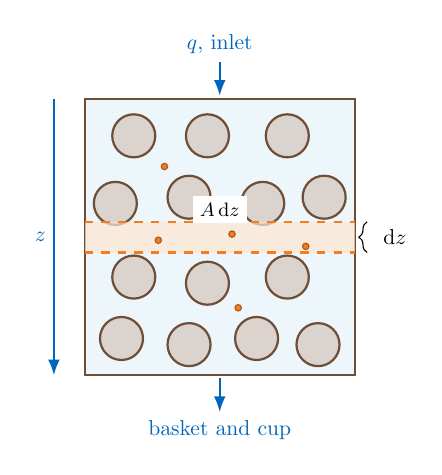
\begin{tikzpicture}[scale=.78,transform shape]
\fill[waterblue!12] (0,0) rectangle (4.4,4.5);
\draw[thick,coffee] (0,0) rectangle (4.4,4.5);
\foreach \x/\y in {.6/.6,1.7/.5,2.8/.6,3.8/.5,.8/1.6,2/1.5,3.3/1.6,.5/2.8,1.7/2.9,2.9/2.8,3.9/2.9,.8/3.9,2/3.9,3.3/3.9}{\node[grain,minimum size=7mm] at (\x,\y) {};}
\fill[tumorange!20,opacity=.7] (0,2.0) rectangle (4.4,2.5);
\draw[tumorange,thick,dashed] (0,2)--(4.4,2);
\draw[tumorange,thick,dashed] (0,2.5)--(4.4,2.5);
\draw[decorate,decoration={brace,amplitude=3pt}] (4.6,2)--(4.6,2.5) node[midway,right=4pt] {$\mathrm dz$};
\foreach \x/\y in {1.2/2.2,2.4/2.3,3.6/2.1,1.3/3.4,2.5/1.1}{\node[fine] at (\x,\y) {};}
\draw[arr] (2.2,5.1)--(2.2,4.55) node[pos=0,above] {$q$, inlet};
\draw[arr] (-.5,4.5)--(-.5,0) node[midway,left] {$z$};
\draw[arr] (2.2,-.05)--(2.2,-.6) node[below] {basket and cup};
\node[font=\small,fill=white] at (2.2,2.7) {$A\,\mathrm dz$};
\end{tikzpicture}
\column{.48\textwidth}\small
\hi{Water-filled pore space}
\[\mathrm dM_m=\varepsilon c A\,\mathrm dz\]
Mobile fines cross the slice boundaries by advection and dispersion.
\par\medskip
\hi{Stationary coffee skeleton}
\[\mathrm dM_a=m_a A\,\mathrm dz,\quad\mathrm dM_d=m_d A\,\mathrm dz\]
Release and capture exchange fines locally between water and skeleton.
\end{columns}
\vfill\takeaway{The highlighted slice defines the continuum balance. It is not a numerical cell.}
\end{frame}

\begin{frame}{Continuum equations and optional surface loading}
\small

\begin{align*}
\frac{\partial(\varepsilon c)}{\partial t}+\frac{\partial(qc)}{\partial z}
 &=\frac{\partial}{\partial z}\left(\varepsilon D\frac{\partial c}{\partial z}\right)
 +R_{\mathrm{rel}}-R_{\mathrm{dep}}+R_{\mathrm{rem}},\\
\frac{\partial m_a}{\partial t}&=-R_{\mathrm{rel}},\qquad
\frac{\partial m_d}{\partial t}=R_{\mathrm{dep}}-R_{\mathrm{rem}}.
\end{align*}
\hi{Equivalent surface description}
\[
 m_a=\sigma c_a,\qquad m_d=\sigma c_d,\qquad
 [\sigma]=\mathrm{m^2/m^3_{bulk}},\quad[c_a]=[c_d]=\mathrm{kg/m^2}.
\]
Use $\partial_t(\sigma c_a)$ if the specific surface area changes.
\vfill
\takeaway{Only mobile fines travel axially. All $R$ terms have units kg/(m$^3_{bulk}$ s).}

\end{frame}

\begin{frame}{Release and capture are constitutive hypotheses}
\small

\hi{Release of initially attached fines}
\[
R_{\mathrm{rel}}=k_{\mathrm{rel}}m_a(|q|/q_{\mathrm{ref}})^{a_r},
\qquad [k_{\mathrm{rel}}]=\mathrm{s^{-1}}.
\]
\hi{Capture of mobile fines}
\[
R_{\mathrm{dep}}=k_{\mathrm{dep}}\chi(z)|q|c
\left[1-\frac{m_d}{m_{\mathrm{cap}}}\right]_+,
\qquad[k_{\mathrm{dep}}]=\mathrm{m^{-1}}.
\]
\begin{itemize}
\item Release depends on the remaining available inventory and flow.
\item Capture depends on mobile flux and available deposit capacity.
\item $\chi=1$ is the unbiased baseline. Axial weighting needs evidence.
\item Compare these laws using multiple flow rates and spatial deposit data.
\end{itemize}

\end{frame}

\begin{frame}{Deposit remobilization and local pore accessibility}
\small
\hi{Deposits return to the water only above a forcing threshold}
\[
R_{\mathrm{det}}^*=k_{\mathrm{det}}m_d
\left[\frac{G}{G_{\mathrm{crit}}}-1\right]_+^b,\qquad
G=\left|\frac{\partial p}{\partial z}\right|.
\]
At $G\leq G_{\mathrm{crit}}$, remobilization is zero. Above the threshold,
more deposits and stronger forcing increase the potential detachment rate.
\[
R_{\mathrm{rem}}=P_{\mathrm{mob}}R_{\mathrm{det}}^*,\qquad
P_{\mathrm{mob}}=\frac{1}{1+\exp[s(d_f/d_h-\lambda_c)]}.
\]
\begin{itemize}
\item $P_{\mathrm{mob}}$: fraction that can enter flowing pores locally.
\item Larger fines $d_f$ relative to pore diameter $d_h$ reduce this fraction.
\item $\lambda_c$: size ratio at 50\% access. $s$: transition steepness.
\item The remaining fraction stays deposited. Mobile fines may deposit again.
\end{itemize}
\slidesource{Notation: $R_{\mathrm{rem}}=R_{\mathrm{wash}}$ and $P_{\mathrm{mob}}=P_{\mathrm{esc}}$ in the code. The logistic law is an unvalidated closure.}
\end{frame}

\begin{frame}{Fines leaving the puck: sieve retention and cup collection}
\small
\hi{The outlet carries mobile fines out of the puck}
\[
\dot M_{\mathrm{out}}(t)=Q(t)c(L,t)\qquad [\mathrm{kg/s}].
\]
$c(L,t)$ is the fines concentration at the puck outlet.
The outlet model neglects dispersive exchange with the basket.
\par\medskip
\begin{columns}[T,onlytextwidth]
\column{.48\textwidth}\hi{Retained by the sieve}
\[
\dot M_{\mathrm{sieve}}=\eta_s\dot M_{\mathrm{out}}
\]
The basket retains the fraction $\eta_s$ of the outgoing fines.
\column{.48\textwidth}\hi{Collected in the cup}
\[
\dot M_{\mathrm{cup}}=(1-\eta_s)\dot M_{\mathrm{out}}
\]
The remaining fraction passes through the basket into the cup.
\end{columns}
\[
M_j(t)=\int_0^t\dot M_j(\tau)\,\mathrm d\tau,\quad
j\in\{\mathrm{out},\mathrm{sieve},\mathrm{cup}\},\qquad
M_{\mathrm{out}}=M_{\mathrm{sieve}}+M_{\mathrm{cup}}.
\]
\small Zero initial collected masses. The illustrative runs use constant
$\eta_s=0.35$, so 65\% reaches the cup.
\slidesource{Retention $\eta_s$ requires calibration. It differs from hydraulic resistance $R_s$.
In the current model, sieve loading does not change $R_s$.}
\end{frame}

\begin{frame}{The PSD is reduced to quantities used by the 1D closures}
 \begin{columns}[T,onlytextwidth]
  \column{.45\textwidth}{\hi{Measured bimodal PSD}
   \begin{itemize}\item Fit a five-parameter mixture model.
   \item Choose a mobility cutoff $d_{\mathrm{cut}}$.
   \item Estimate the fine fraction and its releasable share.
   \item Calculate representative fine and coarse diameters.\end{itemize}}
  \column{.51\textwidth}{\centering
   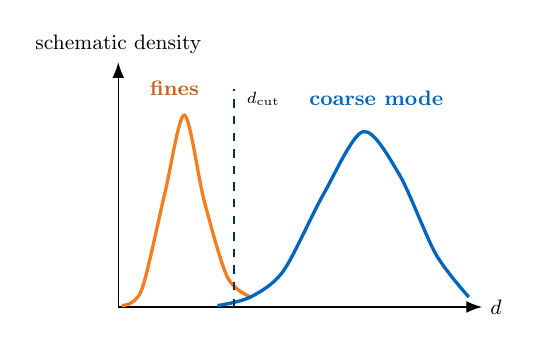
\begin{tikzpicture}[x=1cm,y=1cm,scale=.84,transform shape]
    \draw[-{Latex[length=2mm]}] (0,0)--(5.5,0) node[right,font=\small] {$d$};
    \draw[-{Latex[length=2mm]}] (0,0)--(0,3.7) node[above,font=\small] {schematic density};
    \draw[tumorange,very thick,smooth] plot coordinates{(.05,.02)(.35,.25)(.7,1.7)(1.0,2.9)(1.3,1.6)(1.65,.45)(2.0,.15)};
    \draw[tumblue,very thick,smooth] plot coordinates{(1.5,.02)(2.0,.15)(2.5,.55)(3.1,1.7)(3.7,2.65)(4.25,2.0)(4.8,.8)(5.3,.15)};
    \draw[dashed,tumdark] (1.75,0)--(1.75,3.3);
    \node[font=\scriptsize,anchor=west] at (1.82,3.15) {$d_{\mathrm{cut}}$};
    \node[tumorange!80!black,font=\small\bfseries] at (.85,3.3) {fines};
    \node[tumblue,font=\small\bfseries] at (3.9,3.15) {coarse mode};
   \end{tikzpicture}}
 \end{columns}
 \medskip\small
 \textbf{Use in the model:} the fine mass fraction and its releasable share set the
 initial attached inventory $m_{a,0}$. The fine diameter $d_f$ controls local
 pore access. A representative bed diameter helps estimate the initial pore size.
 \slidesource{Source: Bora and Briesen, Journal of Food Process Engineering 49 (2026), e70645.}
\end{frame}

\begin{frame}{Constant pressure or PI control}
\small
\hi{Constant pressure: controlled reference}
\[
\Delta p_{\mathrm{total}}=9\ \mathrm{bar},\qquad
Q=\Delta p_{\mathrm{total}}/R_{\mathrm{tot}}(t).
\]
The source supplies whatever flow maintains 9 bar. This represents an
experimental 9 bar plateau only when the machine can sustain that pressure.
\par\medskip
\hi{Flow-limited PI: machine--puck prediction}
\[
e=p_{\mathrm{set}}-\Delta p_{\mathrm{total}},\qquad Q_{\mathrm{command}}\leq Q_{\max}.
\]
The controller adjusts pump flow, with feedforward and pump lag.
A permeable puck may stay below the target because the pump reaches its flow limit.
\par\medskip
\takeaway{PI represents machine constraints. Its predictive value requires representative pump limits and controller settings.}
\end{frame}

\begin{frame}{Pressure reference and experimental comparison}
\small
\hi{Our priority: validate flow and cup fines using measured pressure}
\begin{itemize}
\item Prescribe the actual pressure drop to test the puck model without fitting uncertain machine-control parameters.
\item Constant 9 bar is the reference for a sustained 9 bar interval. Use the actual pressure for experiments below the target.
\item Retain flow-limited PI to predict pressure and flow for different initial PSDs, with a representative machine model.
\end{itemize}
\medskip
$p_{\mathrm{out}}=0$, $p_{\mathrm{puck\ exit}}=Q R_s$.
The measured pressure must refer to the same endpoints as the model.
\par\medskip
\takeaway{Measured pressure for validation. PI for machine--puck prediction. Constant 9 bar for comparison.}
\slidesource{Measured time-series input remains an extension. The current saturated-puck model excludes initial wetting.}
\end{frame}

\begin{frame}{Boundary conditions for clean feed and an open outlet}
\small
\[J=qc-\varepsilon D\,\partial_zc\]
\begin{columns}[T,onlytextwidth]
\column{.48\textwidth}\hi{Inlet: no fines supplied}
\[J(0,t)=q c_{\mathrm{in}}=0\]
The feed is clean water. We prescribe the total incoming fines flux.
\par\medskip
This does not require imposing both $c=0$ and $\partial_zc=0$ on the interior solution.
\column{.48\textwidth}\hi{Outlet: convective removal}
\[\partial_zc(L,t)=0,\quad J(L,t)=qc(L,t)\]
We neglect dispersive exchange with the downstream basket/cup region.
\par\medskip
This open-outlet approximation allows fines to leave by advection, without a modeled downstream concentration field.
\end{columns}
\vfill
\small In the code, boundary dispersive fluxes are omitted; inlet total flux is zero and outlet flux is $qc$. Reconsider this closure if downstream mixing or back-dispersion matters.
\end{frame}

\section[Numerics]{Numerical solution and verification}
\begin{frame}{}
\vfill
{\large\color{tumgray}Section 4 of 7}\par\vspace{0.4cm}
{\LARGE\color{tumblue}\textbf{Numerical solution and verification}}\par\vspace{0.5cm}
{\large Algebraic Darcy hydraulics and finite-volume fines transport}
\vfill
\end{frame}

\begin{frame}{Darcy flow follows from the current hydraulic resistance}
\small
\hi{At each update, use the current cell permeabilities $K_i(t)$}
\[
R_{\mathrm{puck}}=\frac{1}{A}\int_0^L\frac{\mu}{K(z,t)}\,\mathrm dz
\;\approx\;\frac{\mu}{A}\sum_i\frac{\Delta z_i}{K_i},
\qquad R_{\mathrm{tot}}=R_s+R_{\mathrm{puck}}.
\]
\begin{tabular}{@{}>{\raggedright\arraybackslash}p{3cm}p{8.9cm}@{}}
\toprule
Operating mode & Algebraic hydraulic evaluation\\\midrule
Pressure imposed & $Q=\Delta p_{\mathrm{total}}/R_{\mathrm{tot}}$\\[.6em]
Flow imposed & $\Delta p_{\mathrm{total}}=Q R_{\mathrm{tot}}$\\[.6em]
PI control & Pump dynamics supply $Q(t)$, then $\Delta p_{\mathrm{total}}=Q(t)R_{\mathrm{tot}}$.\\\bottomrule
\end{tabular}
\par\medskip
\small $R$ has units Pa\,s/m$^3$. The cell sum evaluates the resistance integral.
\vfill\takeaway{Darcy hydraulics use algebraic relations. FVM advances the fines-transport balance.}
\end{frame}

\begin{frame}{Velocity and pressure profiles follow from Darcy}
\small
\begin{columns}[T,onlytextwidth]
\column{.46\textwidth}
\hi{Velocity from the common flow rate}
\[
q(t)=\frac{Q(t)}{A},\qquad
u_{\mathrm{pore},i}(t)=\frac{q(t)}{\varepsilon_i(t)}.
\]
$q$ is the superficial velocity, uniform along the constant-area puck.
\par\medskip
The local pore velocity changes with porosity.
\column{.50\textwidth}
\hi{Pressure from the local resistance}
\[
G_i=\frac{\mu q}{K_i},\qquad p(L)=Q R_s.
\]
\[
p_{i-1/2}=p_{i+1/2}+G_i\Delta z_i.
\]
Starting at the basket, accumulate each cell's pressure loss upstream.
\end{columns}
\medskip
\small Pressures are relative to the cup outlet. The recurrence gives face pressures, with cell pressure at the midpoint for a cellwise constant gradient.
\vfill\takeaway{Numerical quadrature reconstructs pressure. No separate momentum or pressure PDE is solved.}
\end{frame}

\begin{frame}{The finite-volume method enforces flux balance cell by cell}
 \centering
 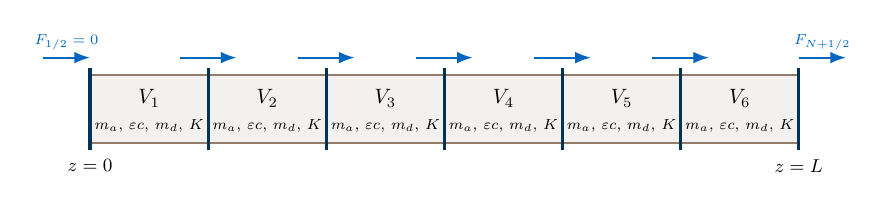
\begin{tikzpicture}[x=1cm,y=1cm,scale=.75,transform shape,
  cell/.style={fill=coffee!8,draw=coffee!75,thick},
  face/.style={very thick,tumdark},
  flux/.style={-{Latex[length=2mm]},thick,tumblue}]
  \draw[flux] (-.8,1.45)--(0,1.45) node[midway,above,font=\scriptsize] {$F_{1/2}=0$};
  \foreach \i [evaluate=\i as \x using 2*(\i-1)] in {1,...,6}{
    \draw[cell] (\x,0) rectangle ({\x+2},1.15);
    \node at ({\x+1},.76) {$V_{\i}$};
    \node[font=\scriptsize] at ({\x+1},.30) {$m_a,\,\varepsilon c,\,m_d,\,K$};}
  \foreach \x in {0,2,4,6,8,10,12}{\draw[face] (\x,-.12)--(\x,1.28);}
  \foreach \x in {2,4,6,8,10}{\draw[flux] ({\x-.48},1.45)--({\x+.48},1.45);}
  \draw[flux] (12,1.45)--(12.8,1.45) node[midway,above,font=\scriptsize] {$F_{N+1/2}$};
  \node[font=\small] at (0,-.38) {$z=0$};
  \node[font=\small] at (12,-.38) {$z=L$};
 \end{tikzpicture}
 \vspace{.15cm}

\[
\frac{(\varepsilon c)_i^{n+1}-(\varepsilon c)_i^n}{\Delta t}
=
-\frac{F_{i+1/2}-F_{i-1/2}}{\Delta z}
+R_{\mathrm{rel},i}-R_{\mathrm{dep},i}+R_{\mathrm{rem},i}.
\]

\[
F_{i+1/2}
=
\underbrace{q\,c_i}_{\text{advection}}
-
\underbrace{
	\varepsilon_{i+1/2}D
	\frac{c_{i+1}-c_i}{\Delta z}
}_{\text{dispersion}},
\qquad q\geq 0.
\]

\small
First-order upwind advection and centred dispersion. No high-order flux limiter.
\par\medskip Shared face fluxes cancel between adjacent cells, preserving the global mass balance.
\end{frame}

\begin{frame}{Why finite volumes for fines transport?}
\small
\hi{The main requirement is consistent mass accounting}
\begin{itemize}
\item Each cell stores a fines inventory and exchanges mass through its faces.
\item One shared face flux leaves one cell and enters the next.
\item Summing the cells cancels internal fluxes; boundary fluxes give collected fines.
\item Local release, capture and remobilization transfer mass between inventories.
\end{itemize}
\medskip
\begin{tabular}{p{2.5cm}p{9cm}}
\toprule
Alternative & Assessment for this model\\\midrule
Finite differences & Equally viable in conservative flux form; on a uniform grid, they can give the same update.\\\bottomrule
\end{tabular}
\vfill\takeaway{FVM is a transparent first implementation. Its first-order upwind diffusion requires grid refinement.}
\end{frame}

\begin{frame}{The smallest timescale limits the numerical step}
\small
\[
\Delta t=\min\left(\Delta t_{\max},\Delta t_{\mathrm{transport}},
\Delta t_{\mathrm{pump}},t_{\mathrm{end}}-t\right)
\]
\[\Delta t_{\mathrm{transport}}=\frac{0.42}{|q|/(\varepsilon_{\min}\Delta z)+2D/\Delta z^2}\]
\begin{tabular}{p{3.5cm}p{8cm}}
\toprule
Limit & Purpose\\\midrule
$\Delta t_{\max}$ & User-selected upper bound for temporal resolution.\\[.5em]
$\Delta t_{\mathrm{transport}}$ & Combined explicit advection--dispersion restriction. Here $\varepsilon_{\min}=\min_i\varepsilon_i(t)$.\\[.5em]
$\Delta t_{\mathrm{pump}}=\tau_p/4$ & Used only in PI mode to resolve pump response; this is not the PI integral time.\\[.5em]
$t_{\mathrm{end}}-t$ & Stops exactly at the requested final time.\\\bottomrule
\end{tabular}
\vfill\small For $D=0$: $\mathrm{Co}=|q|\Delta t/(\varepsilon_{\min}\Delta z)\leq0.42$.
Timestep refinement still checks accuracy of kinetics and coupling. The transport bound is the implemented estimate, not a general heterogeneous-field proof.
\end{frame}

\begin{frame}{Coupled physics and its numerical update}
 \vspace{.25cm}
 \centering
 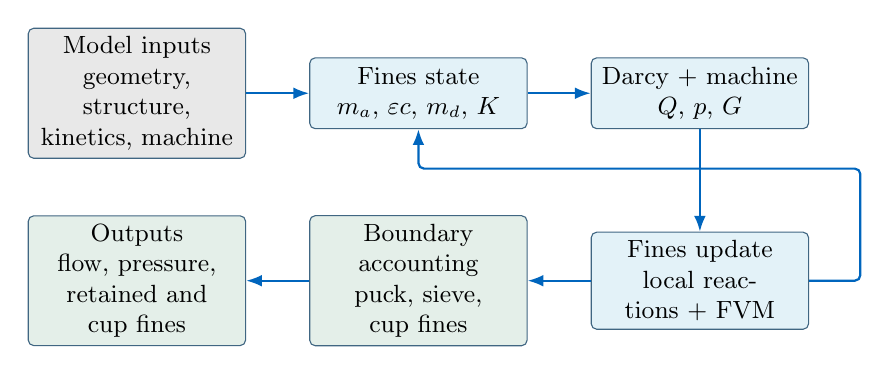
\begin{tikzpicture}[node distance=5mm and 8mm]
  \node[databox] (inputs) {Model inputs\\geometry, structure, kinetics, machine};
  \node[physicsbox,right=of inputs] (state) {Fines state\\$m_a$, $\varepsilon c$, $m_d$, $K$};
  \node[physicsbox,right=of state] (hyd) {Darcy + machine\\$Q$, $p$, $G$};
  \node[physicsbox,below=13mm of hyd] (update) {Fines update\\local reactions + FVM};
  \node[outputbox,left=of update] (basket) {Boundary accounting\\puck, sieve, cup fines};
  \node[outputbox,left=of basket] (outputs) {Outputs\\flow, pressure, retained and cup fines};
  \draw[arr] (inputs)--(state); \draw[arr] (state)--(hyd);
  \draw[arr] (hyd)--(update); \draw[arr] (update)--(basket);
  \draw[arr] (basket)--(outputs);
  \draw[arr,rounded corners=2pt] (update.east)--++(.65,0)
    |- ([yshift=-5mm]state.south)--(state.south);
 \end{tikzpicture}
 \vspace{.35cm}
 \par\vspace{.15cm}
 \small\centering \textbf{Physical coupling:} deposit changes $\varepsilon$, $K$ and $d_h$; these change pressure and flow; the new hydraulics then alter release, deposition and washout.
 \takeaway{Quasi-steady flow is a physical assumption. Update ordering is a numerical choice.}
\end{frame}

\begin{frame}{Numerical verification and physical validation}
\small

\begin{columns}[T,onlytextwidth]
\column{.48\textwidth}\hi{Verification}
\begin{itemize}
\item Conservation and nonnegative inventories.
\item Analytical hydraulic limiting cases.
\item Grid and timestep convergence.
\item Controller limits and boundary accounting.
\end{itemize}
\column{.48\textwidth}\hi{Validation}
\begin{itemize}
\item Pressure and flow measurements.
\item CT structural changes.
\item Collected fines and size distributions.
\item Predictions for withheld cases.
\end{itemize}
\end{columns}
\vfill
\small Current unit tests: 17/17 passed. The four pressure-mode runs conserve fines mass to relative error below $2.1\times10^{-15}$. Physical validation remains outstanding.

\end{frame}

\section[Results]{Illustrative results and model sensitivity}
\begin{frame}{}
\vfill
{\large\color{tumgray}Section 5 of 7}\par\vspace{0.4cm}
{\LARGE\color{tumblue}\textbf{Illustrative results and model sensitivity}}\par\vspace{0.5cm}
{\large How strongly do the hydraulic and permeability choices matter?}
\vfill
\end{frame}

\begin{frame}{Darcy gives practically the same results}
\small
We ran the same case twice, changing only the flow law.
\par\medskip
\begin{center}
\begin{tabular}{lcc}
\toprule
\textbf{Result at 60 s} & \textbf{Darcy--Forchheimer} & \textbf{Darcy}\\\midrule
Pressure [bar] & 8.9905 & 8.9905\\[.8em]
Flow rate [mL/s] & 0.05212 & 0.05212\\[.8em]
Cup fines [g] & 0.03720 & 0.03720\\\bottomrule
\end{tabular}
\par\medskip
{\footnotesize Values rounded for display.}
\end{center}
\medskip
Across the entire simulation, the largest pressure difference was only \textbf{0.0186 Pa}.
\vfill\takeaway{We therefore use Darcy for this tested case.}
\slidesource{Controlled 60 s simulations with identical exponential permeability, kinetics and PI settings.}
\end{frame}

\begin{frame}{The illustrative case develops strong viscous blockage}
{\small\color{tumblue}Constant 9 bar across puck + basket. Exponential permeability.}\par\medskip
 \begin{columns}[T,onlytextwidth]
  \column{.66\textwidth}{\centering\safeimage{hydraulic_response.png}{\linewidth}{3.85cm}}
  \column{.30\textwidth}{\small
   \hi{At 60 s}
   \begin{itemize}\item total pressure: 9.00 bar;
   \item flow: 0.0514 mL/s;
   \item minimum $K/K_0$: 0.0143.\end{itemize}
   \vspace{.25cm}
   \hi{Interpretation}

   At fixed 9 bar, deposition increases resistance and reduces flow. No PI controller is needed.}
 \end{columns}
 \slidesource{New Darcy baseline: exponential permeability, constant 9 bar. Illustrative parameters, no experimental calibration.}
\end{frame}

\begin{frame}{The model distinguishes puck washout from fines in the cup}
{\small\color{tumblue}Constant 9 bar across puck + basket. Exponential permeability.}\par\medskip
 \begin{columns}[T,onlytextwidth]
  \column{.61\textwidth}{\centering\safeimage{fines_washout.png}{\linewidth}{3.85cm}}
  \column{.35\textwidth}{\small
   \hi{Cumulative masses}
   \begin{itemize}\item puck outlet: 0.0577 g;
   \item basket retained: 0.0202 g;
   \item cup: 0.0375 g.\end{itemize}
   \vspace{.25cm}
   With $\eta_s=0.35$, the basket retains 35\% of the fines that leave the puck.}
 \end{columns}
 \slidesource{Constant 9 bar Darcy baseline with exponential permeability; constant basket retention.}
\end{frame}

\begin{frame}{The axial fields locate the effective blocking region}
{\small\color{tumblue}Constant 9 bar across puck + basket. Exponential permeability.}\par\medskip
 \begin{columns}[T,onlytextwidth]
  \column{.49\textwidth}{\centering\safeimage{deposited_fines.png}{\linewidth}{3.85cm}}
  \column{.49\textwidth}{\centering\safeimage{relative_permeability.png}{\linewidth}{3.85cm}}
 \end{columns}
 \vspace{.1cm}
 \takeaway{These fields can be compared with interrupted CT reconstructions, but a 1D layer cannot represent lateral channel geometry.}
 \slidesource{Constant 9 bar Darcy baseline with exponential permeability. The later closure comparison retains its original PI settings.}
\end{frame}


\begin{frame}{Porosity profile evolves as fines redistribute}
{\small\color{tumblue}Dry baseline $\varepsilon_0=0.55$ chosen from the CT dry-state level. Constant 9 bar across puck + basket.}\par\medskip
\begin{columns}[T,onlytextwidth]
 \column{.66\textwidth}\centering
  \safeimage{porosity_profiles.pdf}{\linewidth}{4.05cm}
 \column{.30\textwidth}\small
  \hi{Predicted structure}
  \begin{itemize}
   \item Direct model observable: $\varepsilon(z,t)$.
   \item Dry baseline: $\varepsilon_0=0.55$.
   \item Deposition lowers porosity, strongest near outlet/bottom.
   \item At 60 s: $\varepsilon\approx0.529$--$0.544$.
  \end{itemize}
\end{columns}
\vspace{.08cm}
\takeaway{After matching the dry-state baseline, compare magnitude, axial trend and time evolution with interrupted CT profiles.}
\end{frame}

\begin{frame}{Fine puck: constant pressure versus PI}
{\small\color{tumblue}Constant 9 bar vs.\ PI, 9 bar target. Exponential permeability.}\par\medskip
\centering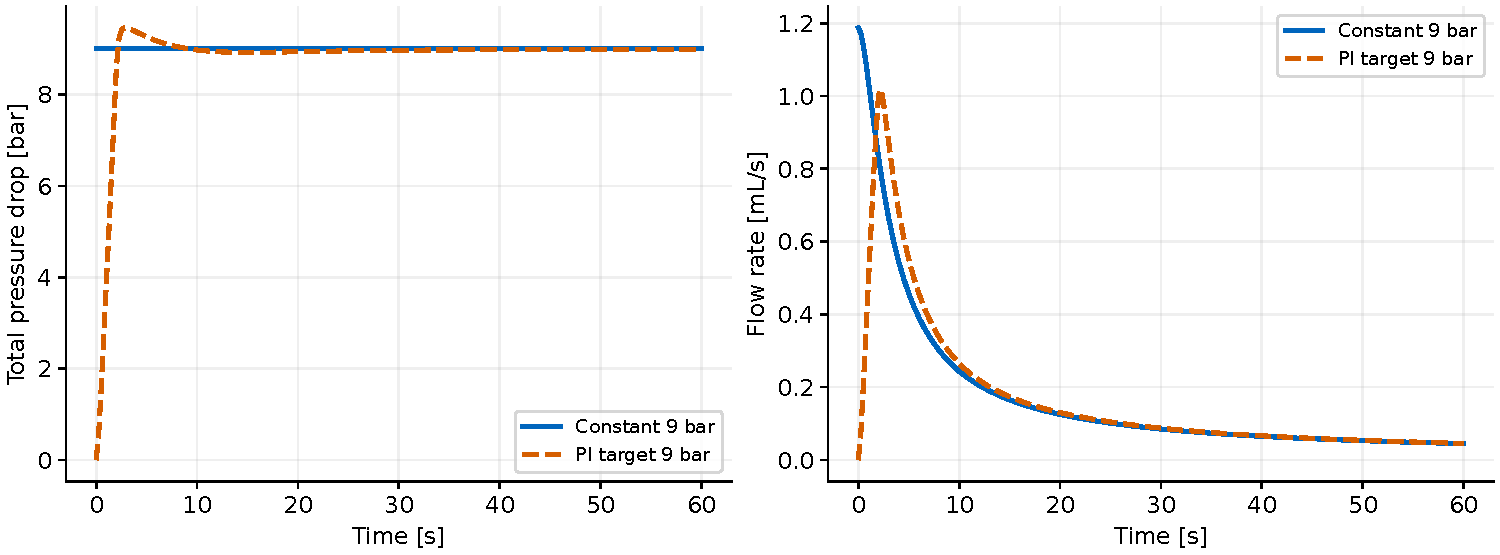
\includegraphics[width=.94\linewidth,height=3.5cm,keepaspectratio]{fine_puck_hydraulics.pdf}
\par\small At 60 s: constant pressure gives $Q=0.0514$ mL/s; PI gives $Q=0.0521$ mL/s. The PI startup ramp changes the earlier fines history.
\slidesource{Matched 60 s runs. Only control mode changes. Darcy + exponential, illustrative parameters.}
\end{frame}

\begin{frame}{Coarse puck: the pump cap limits initial pressure}
{\small\color{tumblue}Constant 9 bar vs.\ PI, 9 bar target. Exponential permeability.}\par\medskip
\centering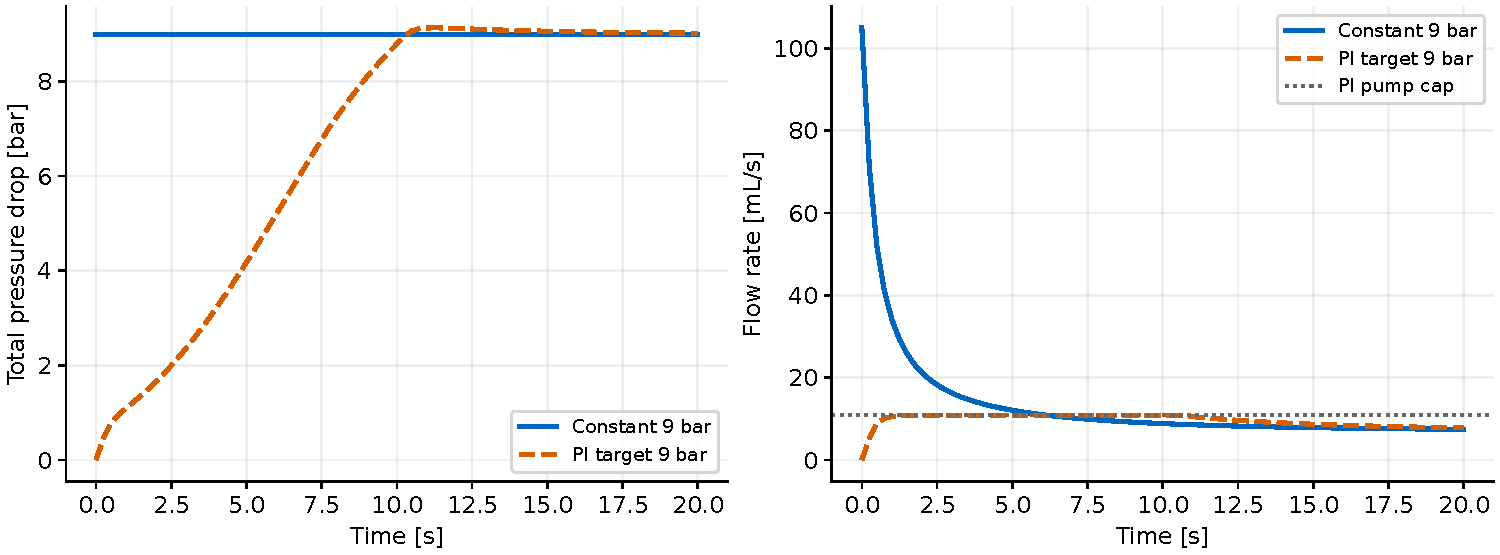
\includegraphics[width=.94\linewidth,height=3.5cm,keepaspectratio]{coarse_puck_hydraulics.pdf}
\par\small Constant 9 bar initially requires 105.0 mL/s, above the PI cap of 10.83 mL/s. PI is initially flow-limited before resistance increases. Deposition later raises resistance enough to reach the target.
\slidesource{Matched 20 s runs with active fines. This coarse case does not stay below 9 bar throughout. No experimental calibration.}
\end{frame}

\begin{frame}{Pressure history also changes fines reaching the cup}
{\small\color{tumblue}Constant 9 bar vs.\ PI, 9 bar target. Exponential permeability.}\par\medskip
\begin{columns}[T,onlytextwidth]
\column{.65\textwidth}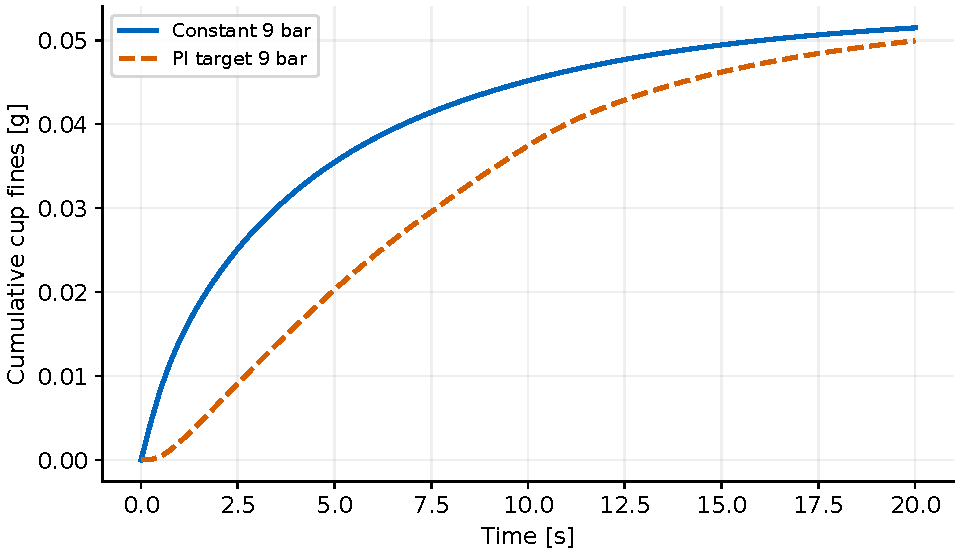
\includegraphics[width=\linewidth,height=3.6cm,keepaspectratio]{coarse_puck_fines.pdf}
\column{.32\textwidth}\small
\hi{Same coarse puck and kinetics}
\par\medskip Different pressure histories change flow, release and deposition.
\par\medskip A fixed 9 bar run cannot directly represent a lower-pressure experiment.
\end{columns}
\slidesource{Only control mode differs. Basket retention and permeability closure are identical.}
\end{frame}

\begin{frame}{Permeability closure strongly changes the flow response}
{\small\color{tumblue}Flow-limited PI, 9 bar target. Exponential vs.\ Kozeny--Carman.}\par\medskip
\begin{columns}[c,onlytextwidth]
\column{.66\textwidth}
\includegraphics[width=\linewidth,height=3.6cm,keepaspectratio]{comparison_flow.pdf}
\column{.31\textwidth}\small\hi{At 60 s}
\par\medskip Exponential:\\$Q=0.0454$ mL/s
\par\medskip Kozeny--Carman:\\$Q=0.892$ mL/s
\par\medskip Both Darcy runs approach the 9 bar PI target.
\end{columns}
\vfill\takeaway{The closure changes resistance and flow, even with nearly the same final pressure.}
\slidesource{Same initial $K_0$, kinetics and machine parameters. Gray and blue curves overlap: inertia is negligible.}
\end{frame}

\begin{frame}{Kozeny--Carman predicts weaker permeability loss}
{\small\color{tumblue}Flow-limited PI, 9 bar target. Exponential vs.\ Kozeny--Carman.}\par\medskip
\begin{columns}[c,onlytextwidth]
\column{.66\textwidth}
\includegraphics[width=\linewidth,height=3.6cm,keepaspectratio]{comparison_permeability.pdf}
\column{.31\textwidth}\small\hi{Minimum $K/K_0$}
\par\medskip Exponential:\\$0.0126$
\par\medskip Kozeny--Carman:\\$0.723$
\par\medskip The same deposit-to-porosity law feeds both closures.
\end{columns}
\vfill\takeaway{The exponential law imposes stronger blockage. The comparison does not establish which closure is correct.}
\slidesource{Final profiles at 60 s. Coupled deposit fields also differ because flow feeds back on kinetics.}
\end{frame}

\begin{frame}{The permeability closure also changes cup fines}
{\small\color{tumblue}Flow-limited PI, 9 bar target. Exponential vs.\ Kozeny--Carman.}\par\medskip
\begin{columns}[c,onlytextwidth]
\column{.66\textwidth}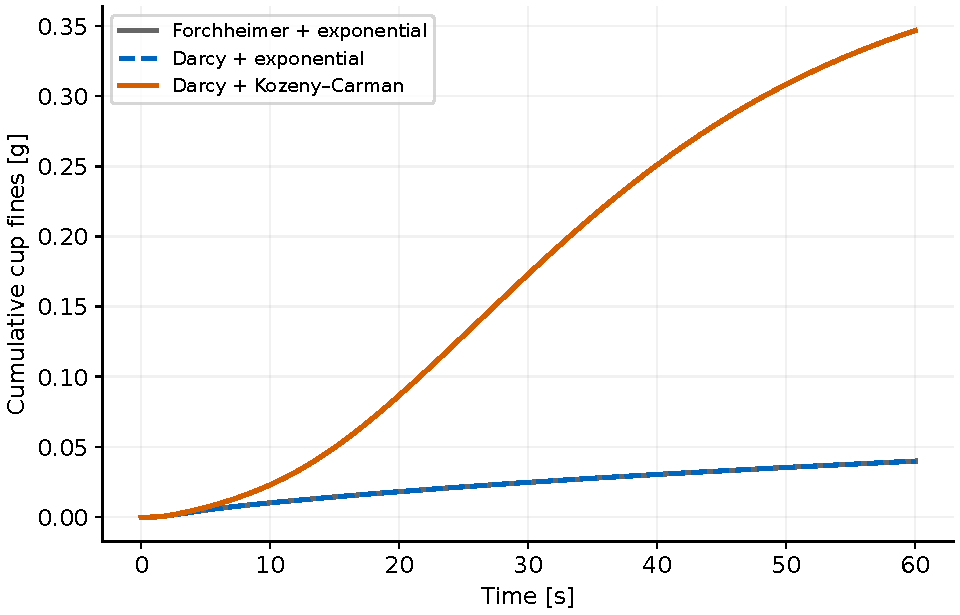
\includegraphics[width=\linewidth,height=3.6cm,keepaspectratio]{comparison_cup_fines.pdf}
\column{.31\textwidth}\small\hi{Cup fines at 60 s}
\par\medskip Exponential:\\$0.0399$ g
\par\medskip Kozeny--Carman:\\$0.3466$ g
\par\medskip Same basket retention:\\$\eta_s=0.35$.
\end{columns}
\vfill\takeaway{This is closure sensitivity, not validation. Neither prediction is an experimental target.}
\slidesource{All kinetic and machine parameters held fixed. No fitting to reproduce the exponential-law result.}
\end{frame}

\section[Calibration]{Calibration and validation strategy}
\begin{frame}{}
\vfill
{\large\color{tumgray}Section 6 of 7}\par\vspace{0.4cm}
{\LARGE\color{tumblue}\textbf{Calibration and validation strategy}}\par\vspace{0.5cm}
{\large Which measurements constrain each part of the model?}
\vfill
\end{frame}

\begin{frame}{Calibration begins with independently measured structure}
\small

\begin{tabular}{p{3cm}p{8.3cm}}
\toprule
Input & Measurement or proposed inference\\\midrule
Geometry and fluid & Puck height and area, temperature-dependent viscosity and density.\\[.6em]
PSD and available fines & Fine fraction, representative sizes and an independently constrained releasable share.\\[.6em]
Initial structure & CT porosity and heterogeneity. Accessible specific surface $\sigma$ with resolution uncertainty.\\[.6em]
Hydraulics & Low-flow pressure--flow slope for $K_0$, empty-basket loss for $R_s$.\\[.6em]
Future pore networks & Connectivity-sensitive permeability and capture/accessibility closures.\\\bottomrule
\end{tabular}
\vfill
\takeaway{CT-derived hydraulic diameter is a structural proxy, not a direct measurement of every pore throat.}

\end{frame}

\begin{frame}{Experiments to distinguish competing kinetic models}
\small

\begin{itemize}
\item Fines collected in time intervals at several flows constrain release and capture.
\item Interrupted CT locates retained material and redistribution.
\item Pressure pulses test deposit remobilization and threshold behavior.
\item Outlet size distributions test size selectivity.
\item Basket-retained mass separates puck transport from cup collection.
\end{itemize}
\medskip
\hi{Model comparisons}
\small One versus two retained populations; accessibility factor versus $P_{\mathrm{mob}}=1$; uniform capture versus axial weighting.
\vfill
\takeaway{These are proposed experiments and comparisons. Validate on withheld pucks or grind settings.}

\end{frame}

\begin{frame}{Next comparison: redistribution versus washout}
\small

\hi{Retained redistribution}
\small Fines release and move, but deposition elsewhere in the puck dominates. CT changes while cumulative outlet mass stays small.
\par\medskip
\hi{Net washout}
\small Mobile fines reach the puck outlet. Basket retention and cup collection quantify the outgoing mass.
\par\medskip
\hi{Proposed study}
\begin{itemize}
\item Compare pressure or flow levels with the same initial puck structure.
\item Record $M_a$, $M_m$, $M_d$ and $M_{\mathrm{out}}$ with axial deposit profiles.
\item Darcy is sufficient here. Compare both permeability predictions with data.
\item Use PNM or 2D/3D only where pore connectivity or radial bypass demands it.
\end{itemize}

\end{frame}

\section[Conclusions]{Conclusions and next steps}
\begin{frame}{}
\vfill
{\large\color{tumgray}Section 7 of 7}\par\vspace{0.4cm}
{\LARGE\color{tumblue}\textbf{Conclusions and next steps}}\par\vspace{0.5cm}
{\large What the model shows and which evidence is still needed}
\vfill
\end{frame}

\begin{frame}{Conclusions and next steps}
\begin{itemize}
\setlength{\itemsep}{.65em}
\item Fines inventories evolve through conservative transport and local exchange.
\item Darcy gives pressure and flow from the evolving hydraulic resistance.
\item Inertia is negligible in the tested case, while permeability closure strongly affects the predictions.
\item Calibration needs independent structure, pressure--flow and fines measurements.
\end{itemize}
\medskip
\takeaway{The next step is to constrain the permeability and kinetic closures with data. Physical validation remains outstanding.}
\end{frame}

\begin{frame}{References and model documentation}
 \small
 \begin{itemize}
  \item M. Bora and H. Briesen, ``Characterization of Bimodal Particle Size Distribution of Ground Coffee Powder,'' \emph{Journal of Food Process Engineering}, 49, e70645, 2026. \texttt{doi:10.1111/jfpe.70645}
  \item S. Ergun, ``Fluid Flow through Packed Columns,'' \emph{Chemical Engineering Progress}, 48, 89--94, 1952.
  \item FineFlow--Espresso technical report, Python solver, named-case configuration and automated verification suite accompanying this presentation.
 \end{itemize}
 %\vspace{.55cm}
% \takeaway{All numerical plots in this presentation were generated by the supplied Python package.}
\end{frame}

\end{document}
